%Este trabalho está licenciado sob a Licença Creative Commons Atribuição-CompartilhaIgual 3.0 Não Adaptada. Para ver uma cópia desta licença, visite http://creativecommons.org/licenses/by-sa/3.0/ ou envie uma carta para Creative Commons, PO Box 1866, Mountain View, CA 94042, USA.

\documentclass[../livro.tex]{subfiles} 


%define o diretório principal
\providecommand{\dir}{..}

%%%%%%%%%%%%%%%%%%%%%%%%%%%%%%%%%%%%%%%%%%%%%
%%%%%%%%%%%%INICIO DO DOCUMENTO%%%%%%%%%%%%%%
%%%%%%%%%%%%%%%%%%%%%%%%%%%%%%%%%%%%%%%%%%%%%

\begin{document}

\chapter{Semana 3}

\section{Dependência e independência linear}

Nós vimos, por definição, que um vetor $\vec{v} \in \mathbb{R}^m$ é combinação linear dos $k$ vetores $\vec{v}_1, \vec{v}_2, \dots, \vec{v}_k  \in \mathbb{R}^m$ quando conseguirmos encontrar números reais $x_1, x_2, \dots, x_k$ tais que
\begin{equation}
x_1 \vec{v}_1 + x_2 \vec{v}_2 + \cdots + x_k \vec{v}_k = \vec{v}.
\end{equation} Vimos também que para decidir se um vetor é combinação linear de outros, devemos verificar se existem estes números reais $x_1, x_2, \dots, x_k$. Em coordenadas, isto é equivalente a resolver o sistema linear:
\begin{equation}
\left[
  \begin{array}{ccccc}
   v_{11} & v_{12} & v_{13} & \cdots & v_{1k}  \\
   v_{21} & v_{22} & v_{23} & \cdots & v_{2k}  \\
   v_{31} & v_{32} & v_{33} & \cdots & v_{3k}  \\
   \vdots & \vdots & \vdots &        & \vdots  \\
   v_{m1} & v_{m2} & v_{m3} & \cdots & v_{mk}  \\
  \end{array}
\right] \left[
  \begin{array}{c}
    x_{1} \\
    x_{2} \\
    x_{3} \\
    \vdots \\
    x_{k} \\
  \end{array}
\right] =
\left[
  \begin{array}{c}
    b_{1} \\
    b_{2} \\
    b_{3} \\
    \vdots \\
    b_{k} \\
  \end{array}
\right].
\end{equation}

Agora, dizemos que os vetores $\vec{v}_1, \vec{v}_2, \dots, \vec{v}_k  \in \mathbb{R}^m$ são \textbf{linearmente independentes (LI)} se nenhum dos vetores puder ser escrito combinação linear dos demais. Uma forma de escrever isto matematicamente é a seguinte:
\begin{equation}
\boxed{\text{Se } x_1 \vec{v}_1 + x_2 \vec{v}_2 + \cdots + x_k \vec{v}_k = \vec{0}, \text{ então } x_1 = x_2 = \cdots = x_k = 0.}
\end{equation} De fato, imaginem que pelo menos um dos coeficientes acima fosse diferente de zero, digamos $x_2 \neq 0$. Daí podemos dividir por $x_2$ e conseguiríamos escrever o vetor $\vec{v}_2$ como combinação linear dos demais:
\begin{equation}
\vec{v}_2 = - \frac{x_1}{x_2} \, \vec{v}_1 - \frac{x_3}{x_2} \, \vec{v}_3 - \cdots - \frac{x_k}{x_2} \, \vec{v}_k.
\end{equation} Se os vetores $\vec{v}_1, \vec{v}_2, \dots, \vec{v}_k  \in \mathbb{R}^m$ não forem linearmente independentes, então nós dizemos que eles são \textbf{linearmente dependentes (LD)}.

\begin{example}\label{exp:1}
Vamos verificar se os vetores
\begin{equation}
\left[
  \begin{array}{c}
    1 \\
    0 \\
    0 \\
  \end{array}
\right], \quad
\left[
  \begin{array}{c}
    1 \\
    1 \\
    0 \\
  \end{array}
\right], \quad
\left[
  \begin{array}{c}
    1 \\
    1 \\
    1 \\
  \end{array}
\right]
\end{equation} são LI ou LD.

Para verificar se são LI, nós devemos considerar a equação vetorial
\begin{equation}
x_1 \left[
  \begin{array}{c}
    1 \\
    0 \\
    0 \\
  \end{array}
\right] +
x_2\left[
  \begin{array}{c}
    1 \\
    1 \\
    0 \\
  \end{array}
\right] +
x_3\left[
  \begin{array}{c}
    1 \\
    1 \\
    1 \\
  \end{array}
\right] = \vec{0} =
\left[
  \begin{array}{c}
    0 \\
    0 \\
    0 \\
  \end{array}
\right].
\end{equation} Como a equação é homogênea, temos pelo menos a solução trivial: $x_1 = 0$, $x_2=0$ e $x_3 = 0$. Se esta for a única solução, então os vetores são LI. Se existir alguma outra solução que não seja a trivial, então os vetores são LD.

Resolver a equação vetorial equivale a resolver o sistema linear
\begin{equation}
\left[
  \begin{array}{ccc}
    1 & 1 & 1 \\
    0 & 1 & 1 \\
    0 & 0 & 1 \\
  \end{array}
\right]
\left[
  \begin{array}{c}
    x_1 \\
    x_2 \\
    x_3 \\
  \end{array}
\right] =
\left[
  \begin{array}{c}
    0 \\
    0 \\
    0 \\
  \end{array}
\right]
\end{equation} É fácil de ver que a única solução deste sistema é a trivial e, portanto, os vetores são LI. Se este sistema não fosse fácil de resolver, deveríamos começar a resolvê-lo por escalonamento, como de costume. $\ \lhd$
\end{example}

\begin{example}\label{exp:2}
Analisamos agora os vetores
\begin{equation}
\left[
  \begin{array}{c}
    1 \\
    0 \\
    1 \\
  \end{array}
\right], \quad
\left[
  \begin{array}{c}
    1 \\
    1 \\
    0 \\
  \end{array}
\right], \quad
\left[
  \begin{array}{c}
    1 \\
    1 \\
    1 \\
  \end{array}
\right], \quad
\left[
  \begin{array}{c}
    -1 \\
    2 \\
    1 \\
  \end{array}
\right].
\end{equation} Como no exemplo anterior, para verificar se são LI, nós devemos considerar a equação vetorial
\begin{equation}
x_1 \left[
  \begin{array}{c}
    1 \\
    0 \\
    0 \\
  \end{array}
\right] +
x_2\left[
  \begin{array}{c}
    1 \\
    1 \\
    0 \\
  \end{array}
\right] +
x_3\left[
  \begin{array}{c}
    1 \\
    1 \\
    1 \\
  \end{array}
\right]+
x_4\left[
  \begin{array}{c}
    -1 \\
    2 \\
    1 \\
  \end{array}
\right] =
\left[
  \begin{array}{c}
    0 \\
    0 \\
    0 \\
  \end{array}
\right].
\end{equation} Como a equação é homogênea, temos pelo menos a solução trivial: $x_1 = 0$, $x_2=0$ e $x_3 = 0$. Se esta for a única solução, então os vetores são LI. Se existir alguma outra solução que não seja a trivial, então os vetores são LD.

Resolver a equação vetorial equivale a resolver o sistema linear
\begin{equation}
\left[
  \begin{array}{cccc}
    1 & 1 & 1 & -1 \\
    0 & 1 & 1 & 2  \\
    1 & 0 & 1 & 1  \\
  \end{array}
\right]
\left[
  \begin{array}{c}
    x_1 \\
    x_2 \\
    x_3 \\
    x_4 \\
  \end{array}
\right] =
\left[
  \begin{array}{c}
    0 \\
    0 \\
    0 \\
  \end{array}
\right].
\end{equation} Em um sistema com mais variáveis do que equações, podemos não ter soluções (no caso de alguma linha inconsistente) ou podemos ter infinitas soluções (no caso de haver variáveis livres). Não é possível ter unicidade. Como já sabemos que em um sistema homogêneo, sempre temos pelo menos a solução trivial $x_1 = 0$, $x_2=0$, $x_3=0$ e $x_4 = 0$, podemos concluir que existem infinitas soluções. Logo, o conjunto de vetores é LD.
\end{example}

O argumento que utilizamos no Exemplo \ref{exp:2} acima é geral e se aplica em várias situações. Temos
\begin{equation}
\boxed{\text{Se $k>m$, então os vetores } \vec{v}_1, \vec{v}_2, \dots, \vec{v}_k  \in \mathbb{R}^m \text{ são necessariamente LD.}}
\end{equation} Desta forma, não existem quatro vetores LI em $\mathbb{R}^3$. Não conseguiríamos encontrar sete vetores LI em $\mathbb{R}^5$ e assim por diante.


Façamos agora algumas observações gerais sobre independência linear:
\begin{itemize}
  \item O vetor nulo, mesmo que sozinho, é LD. Se $\vec{v} = \vec{0}$ estiver em um conjunto de vetores, este conjunto será automaticamente LD.
  \item Ao considerarmos apenas dois vetores $\vec{u}$ e $\vec{v}$, dizer que estes vetores são LD significa que eles são múltiplos um do outro e, portanto, colineares.
  \item Veremos mais adiante no curso que a dimensão do espaço gerado por vetores linearmente independentes é exatamente o número de vetores. Desta maneira, concluiremos, por exemplo, que o conjunto gerado por dois vetores do espaço tridimensional é um espaço linear de dimensão dois: um plano.
\end{itemize}


\section{Independência linear e sistemas lineares}

Na última semana (capítulo anterior), vimos que resolver o sistema linear $A \vec{x} = \vec{b}$ equivale a decidir se o vetor $\vec{b}$ é uma combinação linear das colunas de $A$. Na seção anterior, introduzimos a questão de decidir se os vetores $\vec{v}_1, \vec{v}_2, \dots, \vec{v}_k$ são LI ou LD. Isto, consequentemente\footnote{Lembra que uma equação vetorial pode ser reescrita como uma equação matricial!}, equivale a decidir se existe solução não trivial para o sistema linear homogêneo
\begin{equation}
A \vec{x} = \vec{0},
\end{equation} onde a matriz $A$ é formada com os vetores $\vec{v}_1, \vec{v}_2, \dots, \vec{v}_k$ como colunas.

\begin{example}
Naturalmente, podemos traduzir os exemplos da seção anterior desta forma. Ou seja no Exemplo \ref{exp:1}, temos que a matriz
\begin{equation}
A = \left[
  \begin{array}{ccc}
    1 & 1 & 1  \\
    0 & 1 & 1   \\
    1 & 0 & 1  \\
  \end{array}
\right]
\end{equation} tem as colunas linearmente independentes (LI). Por outro lado, as colunas da matriz
\begin{equation}
B = \left[
  \begin{array}{cccc}
    1 & 1 & 1 & -1 \\
    0 & 1 & 1 & 2  \\
    1 & 0 & 1 & 1  \\
  \end{array}
\right]
\end{equation} do Exemplo \ref{exp:2} são linearmente dependentes (LD). $\ \lhd$
\end{example}

Podemos pensar ainda de outra forma. Considere uma matriz $A$ de ordem $m\times n.$ Para decidir se as colunas de $A$ são LI, devemos procurar por soluções não triviais do sistema linear cuja matriz associada é $A$. Ao resolver um \textbf{sistema homogêneo} por escalonamento, sabemos que
\begin{itemize}
  \item Se existirem mais colunas do que linhas ($i.e. \ m<n$), então as colunas de $A$ são necessariamente LD.
  \item Se existirem mais linhas do que colunas ($i.e. \ m>n$), procedemos por escalonamento. Se todas as colunas da matriz $A$ possuirem posição de pivô, então as colunas são LI (pois daí a única solução do sistema homogêneo é a trivial). 
  \item No caso de alguma coluna não possuir posição de pivô, o sistema homogêneo possui pelo menos uma variável livre; logo, as colunas de $A$ são LD.
\end{itemize}

\begin{example}
Decidir se as colunas de $A$ são LI:
\begin{equation}
A = \left[
\begin{array}{rrrr}
   2&1&-1&8\\
   -3&-1&2&-11\\
   6&2&-4&22\\
   -2&1&2&-3
\end{array}
\right].
\end{equation} Como as colunas de $A$ são quatro vetores de $\mathbb{R}^4$, pode ser que sejam LI (caso tivesse uma coluna a mais, saberíamos automaticamente serem LD). Aplicando o algoritmo de escalonamento, sabemos que
\begin{equation}
A \sim \left[
\begin{array}{cccc}
   2&1&-1&8\\
   0&1&1&2\\
   0&0&-1&1\\
   0&0&0&0\\
\end{array}
\right].
\end{equation} Notando que a última coluna não possui posição de pivô, concluimos que as colunas de $A$ são LD. Isto pois, neste caso, o sistema linear homogêneo associado, $A \vec{x} = \vec{0}$, cuja matriz aumentada associada é
\begin{equation}
\left[
\begin{array}{cccc|c}
   2&1&-1&8&0\\
   0&1&1&2& 0\\
   0&0&-1&1&0\\
   0&0&0&0&0\\
\end{array}
\right],
\end{equation} possui uma variável livre (e portanto outras soluções que não a trivial). $\ \lhd$
\end{example}



\section{Transformações lineares}


Uma \textbf{transformação linear} é um tipo especial de função que associa um vetor a outro vetor
\begin{equation}
T: \{ \text{vetores} \} \to \{ \text{vetores} \}
\end{equation} e com a propriedade adicional:
\begin{equation}
T\big( a \vec{u} + b \vec{v} \big) = aT(\vec{u}) + bT(\vec{v}), \quad \text{para todos } a, b \in \mathbb{R} \quad \text{e todos } \vec{u}, \vec{v}.
\end{equation}
Em geral, pensamos em uma transformação linear como ``transformando um vetor em outro'' de forma linear, isto é, satisfazendo a propriedade acima.


\begin{example}
A aplicação $T: \mathbb{R}^3 \to \mathbb{R}^3$ dada por $T(\vec{u}) = 3\vec{u}$ é a transformação linear que transforma um vetor de $\mathbb{R}^3$ no vetor que tem o triplo do comprimento. Utilizamos a própria fórmula da transformada para verificar que a tranformação $T$ é de fato linear:
\begin{equation}
T\big( a \vec{u} + b \vec{v} \big) = 3 ( a \vec{u} + b \vec{v} ) = a \cdot 3 \vec{u} + b \cdot 3 \vec{v} = aT(\vec{u}) + bT(\vec{v}). \lhd
\end{equation}
\end{example}


\begin{example}\label{exp:4}
Também é linear a transformação que faz uma rotação de um ângulo $\pi / 2$. Tente se convencer geometricamente que esta transformação é uma transformação linear. Voltaremos a este exmeplo com mais detalhes na seção seguinte$. \ \lhd$
\end{example}



\begin{example}\label{exp:7}
Consideramos a transformação $T: \mathbb{R}^2 \to \mathbb{R}^3$, que transforma vetores de $\mathbb{R}^2$ em vetores de $\mathbb{R}^3$, dada pela fórmula
\begin{equation}
T(x_1, x_2) = (x_1 - 3 x_2, 3x_1 + 5x_2, -x_1 + x_2).
\end{equation} Nota que, excepcionalmente, estamos representando os vetores como linhas. É comum quando tratamos de transformações lineares. Esta fórmula nos diz, por exemplo, que os vetores
\begin{equation}
\vec{u} =
\left[
  \begin{array}{c}
    1 \\
    -1 \\
  \end{array}
\right] \quad \text{e} \quad 
\vec{v} =
\left[
  \begin{array}{c}
    0 \\
    3 \\
  \end{array}
\right]
\end{equation} são transformados nos vetores
\begin{equation}
T\big(\vec{u}\big) =
\left[
  \begin{array}{c}
    1-3\cdot(-1) \\
    3\cdot 1 + 5\cdot(-1) \\
    -1 + (-1)\\
  \end{array}
\right] =
\left[
  \begin{array}{r}
     4 \\
    -2 \\
    -2 \\
  \end{array}
\right] \quad \text{e} \quad
T\big(\vec{v}\big) =
\left[
  \begin{array}{c}
    0-3\cdot 3 \\
    3\cdot 0 + 5\cdot 3 \\
    -0 + 3 \\
  \end{array}
\right] =
\left[
  \begin{array}{r}
    -9 \\
    15 \\
     3 \\
  \end{array}
\right].\lhd
\end{equation}
\end{example}







\section{Matriz de uma transformação linear}


Voltemos à transformação linear
\begin{equation}
T(x_1, x_2) = (x_1 - 3 x_2, 3x_1 + 5x_2, -x_1 + x_2)
\end{equation} do Exemplo \ref{exp:7}. Lembramos que um vetor qualquer de $\mathbb{R}^2$ pode ser escrito como combinação linear dos vetores
\begin{equation}
\vec{e}_1 =
\left[
  \begin{array}{r}
    1 \\
    0 \\
  \end{array}
\right]\quad \text{e}\quad
\vec{e}_2 =
\left[
  \begin{array}{c}
    0\\
    1\\
  \end{array}
\right].
\end{equation} De fato,
\begin{equation}
\vec{u} =
\left[
  \begin{array}{r}
    x_1 \\
    x_2 \\
  \end{array}
\right] =
x_1 \left[
  \begin{array}{r}
    1 \\
    0 \\
  \end{array}
\right] +
x_2 \left[
  \begin{array}{c}
    0\\
    1\\
  \end{array}
\right] = x_1 \vec{e}_1 + x_2 \vec{e}_2.
\end{equation} Logo, utilizando a propriedade de a transformação ser linear, temos que
\begin{equation}
T( \vec{u} ) = T\big( x_1 \vec{e}_1 + x_2 \vec{e}_2 \big) = x_1 T(\vec{e}_1) + x_2 T(\vec{e}_2).
\end{equation} Calculamos $T(\vec{e}_1)$ e $T(\vec{e}_2)$ pela fórmula dada da transformação linear:
\begin{equation}
T(\vec{e}_1) =
\left[
  \begin{array}{r}
    1 \\
    3 \\
    -1 \\
  \end{array}
\right] \quad \text{e}\quad
T(\vec{e}_2) =
\left[
  \begin{array}{r}
    -3 \\
     5 \\
     1 \\
  \end{array}
\right].
\end{equation} Concluimos que
\begin{equation}
T( \vec{u} ) =
x_1 \left[
  \begin{array}{r}
    1 \\
    3 \\
    -1 \\
  \end{array}
\right] + x_2
\left[
  \begin{array}{r}
    -3 \\
     5 \\
     1 \\
  \end{array}
\right] =
\left[
  \begin{array}{rr}
    1  & -3 \\
    3  & 5  \\
    -1 & 1 \\
  \end{array}
\right]
\left[
  \begin{array}{r}
    x_1 \\
    x_2 \\
  \end{array}
\right].
\end{equation} Desta forma, associamos uma matriz de ordem $3 \times 2$ à transformação linear $T: \mathbb{R}^2 \to \mathbb{R}^3$.

O procedimento que aplicamos acima não é particular do exemplo que analisamos, de modo que é sempre possível associar a uma transformação linear $T: \mathbb{R}^n \to \mathbb{R}^m$ uma matriz $A$ de ordem $m\times n$, chamada \textbf{matriz canônica associada à transformação linear} $T$ ou apenas \textbf{matriz associada} a $T$, cujas colunas são os vetores $T(\vec{e}_1), T(\vec{e}_2), T(\vec{e}_3), \dots, T(\vec{e}_n) \in \mathbb{R}^m$ (e portanto $n$ colunas com $m$ componentes cada).


\begin{example}
A transformação linear $T: \mathbb{R}^3 \to \mathbb{R}^3$, $T(\vec{u}) = 5 \vec{u}$, satisfaz
\begin{equation}
T(\vec{e}_1) =
\left[
  \begin{array}{r}
    5 \\
    0 \\
    0 \\
  \end{array}
\right], \quad
T(\vec{e}_2) =
\left[
  \begin{array}{r}
     0 \\
     5 \\
     0 \\
  \end{array}
\right]  \quad \text{e} \quad
T(\vec{e}_3) =
\left[
  \begin{array}{r}
     0 \\
     0 \\
     5 \\
  \end{array}
\right].
\end{equation} Assim, podemos escrever
\begin{equation}
T(\vec{x}) = \left[
  \begin{array}{rrr}
    5  & 0 & 0 \\
    0  & 5 & 0 \\
    0  & 0 & 5 \\
  \end{array}
\right]
\left[
  \begin{array}{r}
    x_1 \\
    x_2 \\
    x_3 \\
  \end{array}
\right]. \lhd
\end{equation}
\end{example}


\begin{example}\label{exp:rotacao}
O método acima pode também ser aplicado para conseguirmos uma fórmula para transformações lineares como as do Exemplo \ref{exp:4}. Vamos considerar a aplicação $T: \mathbb{R}^2 \to \mathbb{R}^2$ definida por
\begin{equation}
T(\vec{x}) = \text{rotação no sentido anti-horário de $\vec{x}$ por um ângulo } \theta \in (0, 2\pi).
\end{equation} A matriz da transformação linear tem por colunas a imagem por $T$ dos vetores $\vec{e}_1$ e $\vec{e}_2$. Observamos que (ver figura)
\begin{figure}[h!]
\begin{center}
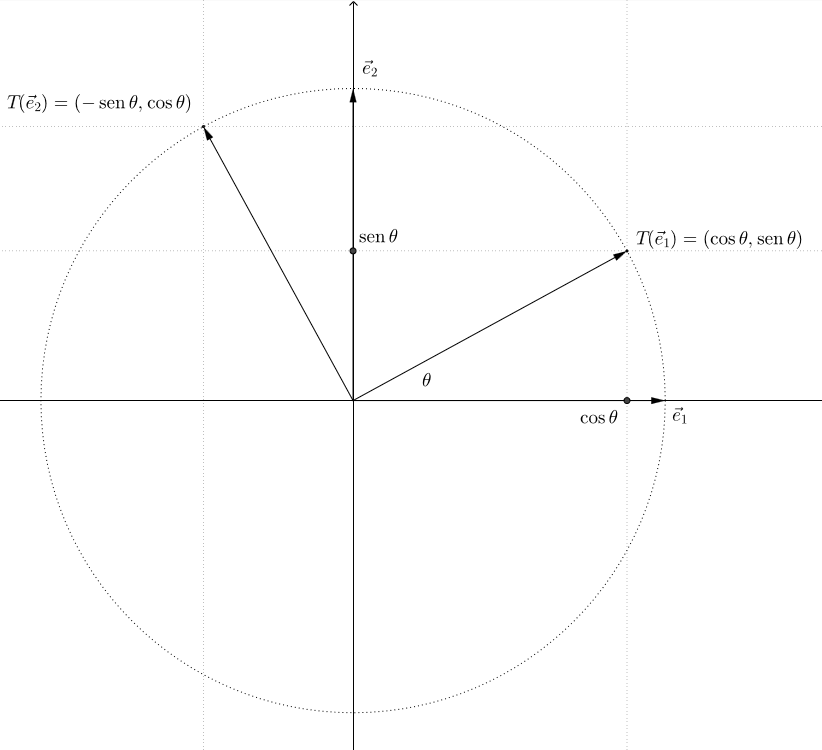
\includegraphics[width=0.8\linewidth]{\dir/Semana03/semana03-rot}
\end{center}
\end{figure}
\begin{equation}
T(\vec{e}_1) =
\left[
  \begin{array}{r}
    \cos \theta \\
    \sen \theta \\
  \end{array}
\right], \quad T(\vec{e}_2) =
\left[
  \begin{array}{r}
    - \sen \theta \\
    \cos \theta \\
  \end{array}
\right].
\end{equation} Logo, concluimos que
\begin{equation}
T(\vec{x}) = \left[
  \begin{array}{rr}
    \cos \theta  & - \sen \theta \\
    \sen \theta  & \cos \theta \\
  \end{array}
\right]
\left[
  \begin{array}{r}
    x_1 \\
    x_2 \\
  \end{array}
\right].
\end{equation}
\end{example}



\section{Transformações injetoras, sobrejetoras e invertíveis}


Como de costume, dada uma função $f: A \to B$, diz-se que $A$ é o domínio de $f$ enquanto $B$ é o contradomínio. A imagem de $f$ é o subconjunto de $B$ que consiste de todos os elementos $y \in B$ tais que $f(x) = y$ ou, intuitivamente, que consiste de ``todos os elementos de $B$ que são atingidos pela função $f$''.

Na hora de decidir se uma função é invertível ou não, duas propriedades são essenciais:
\begin{enumerate}[$1)$]
  \item cada elemento de $B$ ser a imagem de no máximo um elemento de $A$, caso em que $f$ é dita \textbf{injetora} ou \textbf{injetiva};
  \item a imagem de $f$ ser igual ao contradomínio, caso em que $f$ diz-se \textbf{sobrejetora} ou \textbf{sobrejetiva}.
\end{enumerate}

Quando estas duas propriedades são satisfeitas, isto é, quando a função $f$ é injetora e sobrejetora, vale que $f$ é \textbf{invertível}: podemos encontrar uma função $f^{-1} : B \to A$ que satisfaz
\begin{equation}
f^{-1}\big( f (x)\big) = x, \ \text{para todo } x \in A  \quad \text{e} \quad f\big( f^{-1} (y)\big) = y, \ \text{para todo } y \in B.
\end{equation} Ao tentarmos encontrar uma \textbf{função inversa} $f^{-1}$, as propriedades de ser injetora e sobrejetora, aparecem naturalmente.

Estas definições são usuais para funções quaisquer. A partir de agora, vamos analisar quando que transformações lineares são injetoras, sobrejetoras e/ou invertíveis. Vamos ver, em particular, que é bem mais fácil estudar tais propriedades para transformações lineares.

\subsection{Transformações lineares injetoras}

A transformação linear $T: \mathbb{R}^n \to \mathbb{R}^m$ é injetora quando, para $\vec{b} \in \mathbb{R}^m$, a equação
\begin{equation}
T(\vec{x}) = \vec{b}
\end{equation} possuir uma única solução ou nenhuma (no máximo uma -- comparar com a definição acima). Como vimos, existe uma matriz $A$ de ordem $m\times n$ associada à transformação linear $T$, de modo que temos que analisar as soluções de
\begin{equation}
A\vec{x} = \vec{b}.
\end{equation} Recaimos novamente em um sistema linear!

No caso particular em que $\vec{b} = \vec{0}$, o sistema homogêneo $A\vec{x} = \vec{0}$ sempre possui a solução trivial $\vec{x} = \vec{0}$. Neste caso, para que a transformação linear seja injetora devemos verificar que esta é a única solução de $A\vec{x} = \vec{0}$. Na verdade, é possível verificar o seguinte.

% \begin{equation}
% \boxed{\text{$T$ é injetora se, e somente se, $A\vec{x} = \vec{0}$ possui apenas a solução trivial.}}
% \end{equation} Em particular, este caso somente é possível se $n \le m$ (reler observações que seguem o Exemplo 3).


\begin{claim}
  $T$ é injetora se, e somente se, $A\vec{x} = \vec{0}$ possui apenas a solução trivial.\footnote{Em particular, este caso somente é possível se $n \le m$ (reler observações que seguem o Exemplo 3)}
\end{claim}
\begin{proof}[Justificativa da afirmação]
Vamos provar matematicamente que, se soubermos que $A\vec{x} = \vec{0}$ possui apenas a solução trivial, então vale que $A\vec{x} = \vec{b}$ possui no máximo uma solução, para qualquer escolha de vetor $\vec{b}$. Isto, por sua vez, implica que $T$ é injetora. Caso não existam soluções ou caso exista apenas uma, nada há para provar. Suponhamos que então que existem infinitas soluções (esta seria a única outra possibilidade). Em particular, existiriam duas distintas:
\begin{equation}
\vec{x}_1 \neq \vec{x}_2 \text{ tais que } A \vec{x}_1 = \vec{b} \text{ e também } A \vec{x}_2 = \vec{b}.
\end{equation} Por linearidade, temos então que $A (\vec{x}_1 - \vec{x}_2) = \vec{b} - \vec{b} = \vec{0}$. No entanto, nossa hipótese garante que somente existe a solução trivial para a equação $A\vec{x} = \vec{0}$, de modo que deveríamos ter $\vec{x}_1 = \vec{x}_2$. Em outras palavras, se $A\vec{x} = \vec{0}$ possuir apenas a solução trivial, então não existe mais do que uma solução para $A\vec{x} = \vec{b}$. Portanto, $T$ é injetora.
\end{proof}

Notem que a afirmação acima é também equivalente a seguinte afirmação.

% \begin{equation}
% \boxed{\text{$T$ é injetora se, e somente se, as colunas de $A$ são linearmente independentes.}}
% \end{equation} 

\begin{claim}
  $T$ é injetora se, e somente se, as colunas de $A$ são linearmente independentes.
\end{claim}

Vamos deixar exemplos de injetividade para a subseção seguinte (ver Exemplos \ref{exp:injsob1} e \ref{exp:injsob2}).

\subsection{Transformações lineares sobrejetoras}

A transformação linear $T: \mathbb{R}^n \to \mathbb{R}^m$ é sobrejetora quando, para todo $\vec{b} \in \mathbb{R}^n$, a equação
\begin{equation}
T(\vec{x}) = \vec{b}
\end{equation} possui alguma solução (comparar com a definição no início desta seção). Seja $A$ a matriz de ordem $m\times n$ associada a $T$. Assim, para verificar que $T$ é sobrejetora, devemos verificar que, para qualquer $\vec{b} \in \mathbb{R}^m$, o sistema linear
\begin{equation}
A\vec{x} = \vec{b}
\end{equation} possui ao menos uma solução (uma ou infinitas). Isto é equivalente a:


\begin{equation}
\boxed{\text{$T$ é sobrejetora se, e somente se, as colunas de $A$ geram todo o espaço $\mathbb{R}^m$.}}
\end{equation} Em particular, este caso somente é possível se $n \ge m$ (veremos mais adiante no curso -- a imagem da transformação $T: \mathbb{R}^n \to \mathbb{R}^m$ será de dimensão no máximo igual a $n$).


\begin{example}\label{exp:injsob1}
Considere a transformação linear $T$ cuja matriz associada é
\begin{equation}
A = \left[
  \begin{array}{rrrr}
    5  & 3 & 1 & 1 \\
    0  & -1 & 1 & -1 \\
    0  & 0 & 0 & 3 \\
  \end{array}
\right].
\end{equation} Como são quatro colunas de $\mathbb{R}^3$, vemos que as colunas são LD e, portanto, $T$ não é injetora.

Por outro lado, a matriz já está em forma escalonada. Vamos analisar se o sistema
\begin{equation}
A \vec{x} = \vec{b} \iff
\left[
  \begin{array}{rrrr|r}
    5  & 3 & 1 & 1 & b_1\\
    0  & -1 & 1 & -1& b_2\\
    0  & 0 & 0 & 3& b_3\\
  \end{array}
\right]
\end{equation} possui solução para todo $\vec{b} \in \mathbb{R}^3$. De fato, o sistema possui solução (já que nenhuma linha da sua forma escalonada é inconsistente). Em verdade, o sistema possui uma variável livre. Logo, $T$ é sobrejetora.
\end{example}


\begin{example}\label{exp:injsob2}
Considere a transformação linear $T$ cuja matriz associada é
\begin{equation}
A = \left[
  \begin{array}{rrrr}
    3  & 1 \\
    5  & 7 \\
    0  & -4 \\
  \end{array}
\right].
\end{equation} Como são somente duas colunas, é fácil ver que uma não é múltipla da outra: por causa das primeiras componentes, podemos pensar que a primeira coluna é três vezes a primeira, mas verificando a segunda linha já não dá certo $3\cdot 7 \neq 5$. Logo, as colunas são LI e a transformação $T$ é injetora.

Por outro lado,  as colunas de $A$ geram um espaço de dimensão no máximo 2; logo, não geram $\mathbb{R}^3$. Portanto, $T$ não é sobrejetora.
\end{example}


\subsection{Transformações lineares invertíveis}

Pelas observações das últimas subseções, só é possível da transformação linear $T: \mathbb{R}^n \to \mathbb{R}^m$ ser invertível quando $m=n$, pois $T$ deverá ser ao mesmo tempo injetora e sobrejetora. Veremos na semana seguinte um método para calcular a transformação inversa $T^{-1}$, que será também uma transformação linear.

\end{document} 